\chapter{EXPERIMENTAL RESULTS}
We will be analyze our model by there accuracy. Based on the input, or training, data, machine learning model accuracy is the statistic used to discover which model is best at recognizing correlations and patterns between variables in a dataset. The better predictions and insights a model can generate, which in turn provide more commercial value, depend on how well it can generalize to "unseen" data.
\vspace{5pt}
\begin{enumerate}
    \item \textbf{VGG19:} Using VGG-19, the accuracy of cataract vs. normal original data is 97.24\%. Glaucoma vs. normal has an accuracy of 90.94\%. In addition, myopia vs. normal has an accuracy of 98.13\%. The accuracy for hypertensive vs. normal is 94.73\%. It performed very well. We removed bias by balancing images for data classes.
    \vspace{5pt}
    \item \textbf{Resnet50:} Resnet50 is the best performed model according to accuracy. Using Resnet50, the accuracy of cataract vs. normal original data is 99.45\%. Glaucoma vs. normal has an accuracy of 90.98\%. In addition, myopia vs. normal has an accuracy of 99.26\%. The accuracy for hypertensive vs. normal is 94.73\%. It performed very well. We removed bias by balancing images for data classes.
    \vspace{5pt}
     \item \textbf{MobileNetV2:} It is the worst performed model out of three. The result without augmented data is too bad. But after taking augmented data, we did get satisfactory results form this model.
     \begin{enumerate}
         \item Cataract V Normal original data Using MobilenetV2 has 77\% accuracy.
         \item Cataract V Normal augmented data Using MobilenetV2 has 90\% accuracy 
         \item Glaucoma V Normal original data Using MobilenetV2 has 59\% accuracy 
         \item Glaucoma V Normal augmented data Using MobilenetV2 has 84\% accuracy 
         \item Myopia V Normal original data Using MobilenetV2 has 77\% accuracy 
         \item Myopia V Normal augmented data Using MobilenetV2 has 89\% accuracy 
         \item Hypertensive V Normal original data Using MobilenetV2 has 52\% accuracy 
         \item Hypertensive V Normal augmented data Using MobilenetV2 has 88\% accuracy 
     \end{enumerate}
\end{enumerate}
\vspace{5pt}
we can see in the training performance of MobileNetV2, its accuracy is getting improved and it can be inferred that the accuracy will certainly be improved if we run the training for more number of epochs. Also, There is hundred percentage training accuracy issue on VGG19  and Resnet50. We had tried to train those model in various dataset split ratio. There were various issue, but we selected the most optimized one. When we got hundred percentage training accuracy, we looked the accuracy of the model and the curve. If training accuracy curve is above validation curve and the accuracy was the highest, we recorded necessary information. But There is no hundred percent training accuracy issue on MobilenetV2. So, there is no overfitting issue also.\\
\\
\begin{figure}[H]
    \centering
    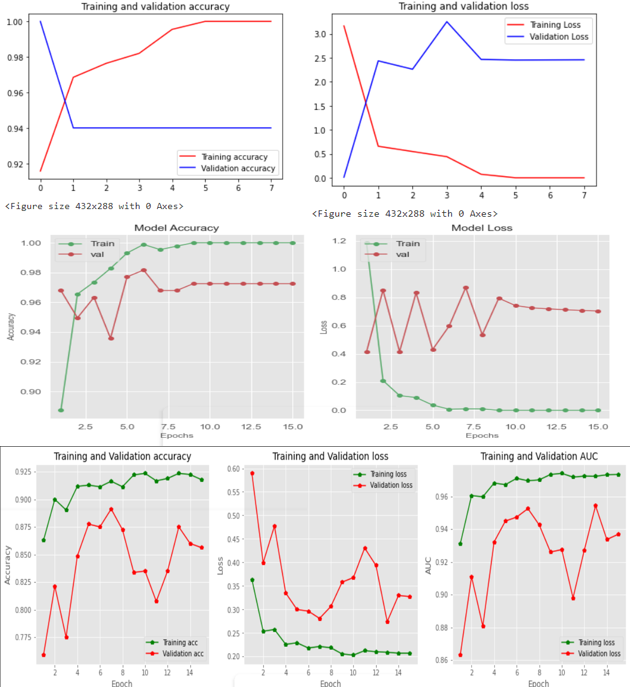
\includegraphics[scale=0.7]{c1.png}
    \caption{Plotting for Cataract v Normal.(Upper: Resnet50, Middle: VGG19, Lower: Mobilenetv2 on Augmented data)}
    \label{Plotting for Cataract v Normal}
\end{figure}
\vspace{5pt}
\\
\begin{figure}[H]
    \centering
    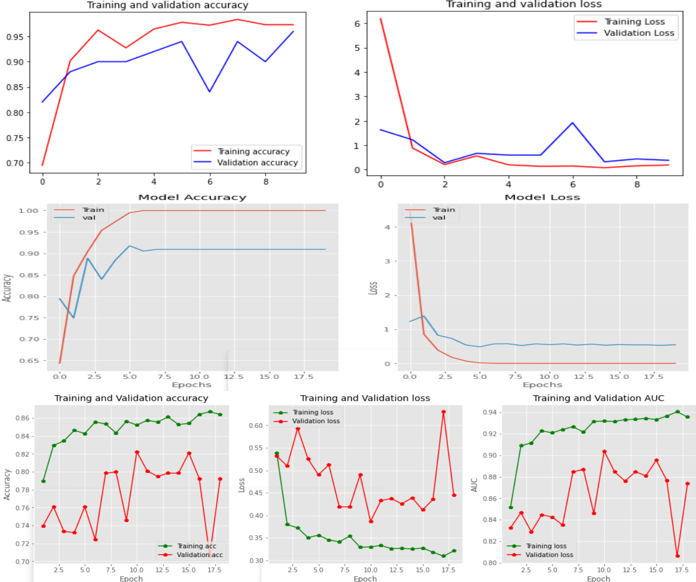
\includegraphics[scale=0.7]{c2.png}
    \caption{Plotting for Glaucoma v Normal.(Upper: Resnet50, Middle: VGG19, Lower: Mobilenetv2 on Augmented data)}
    \label{Plotting for Glaucoma v Normal}
\end{figure}
\vspace{5pt}

\begin{figure}[H]
    \centering
    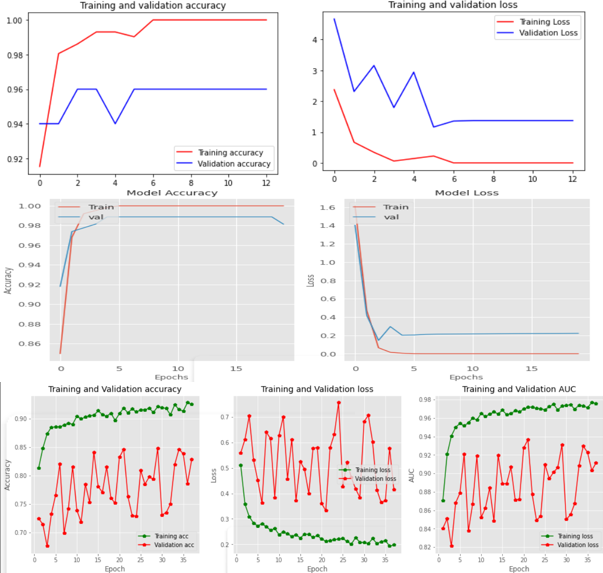
\includegraphics[scale=0.7]{c3.png}
    \caption{Plotting for Myopia v Normal.(Upper: Resnet50, Middle: VGG19, Lower: Mobilenetv2 on Augmented data)}
    \label{Plotting for Myopia v Normal}
\end{figure}
\vspace{5pt}

\begin{figure}[H]
    \centering
    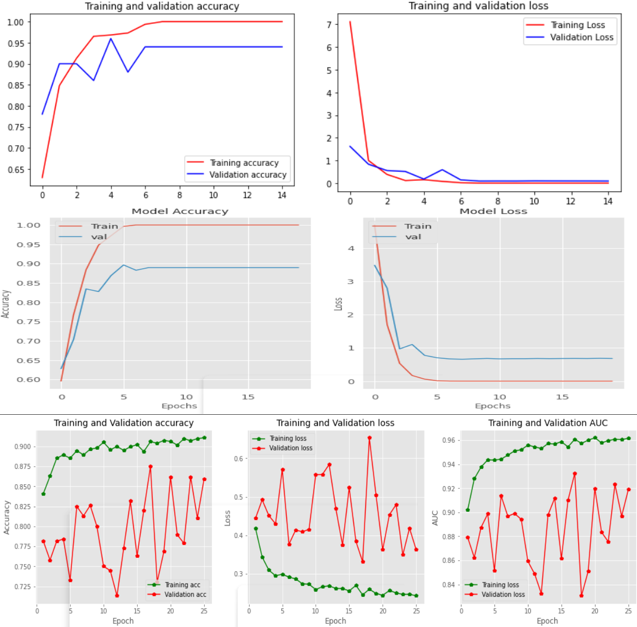
\includegraphics[scale=0.7]{c4.png}
    \caption{Plotting for Hypertensive v Normal.(Upper: Resnet50, Middle: VGG19, Lower: Mobilenetv2 on Augmented data)}
    \label{Plotting for Hypertensive v Normal}
\end{figure}
\begin{figure}[H]
    \centering
    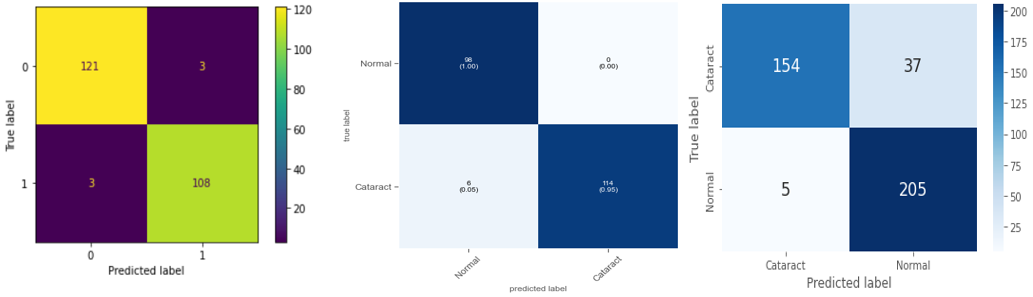
\includegraphics[scale=0.7]{50_Chapter_5/CNC.png}
    \caption{Confusion Matrix for Cataract v Normal.(Left: Resnet50, Middle: VGG19, Right: Mobilenetv2 on Augmented data)}
    \label{CNC}
\end{figure}
\begin{figure}[H]
    \centering
    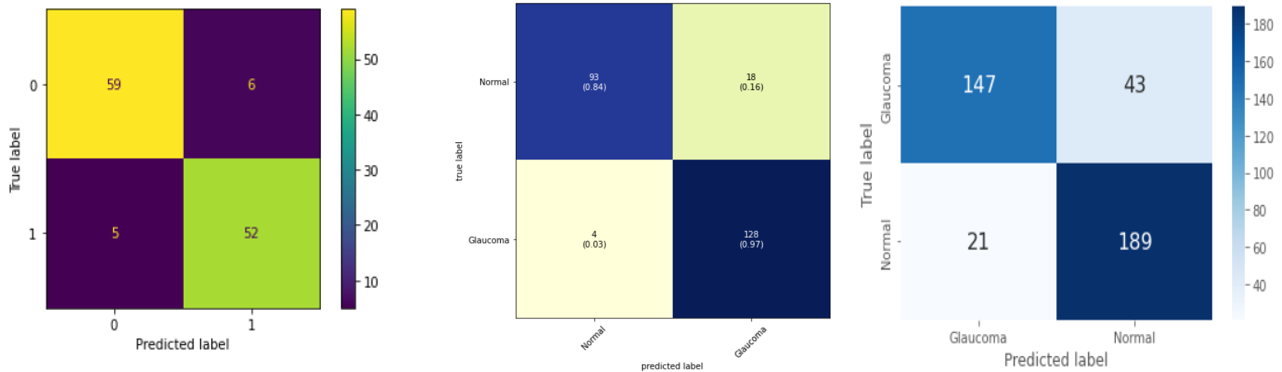
\includegraphics[scale=0.55]{50_Chapter_5/GNC.png}
    \caption{Confusion Matrix for Glaucoma v Normal.(Left: Resnet50, Middle: VGG19, Right: Mobilenetv2 on Augmented data)}
    \label{GNC}
\end{figure}
\begin{figure}[H]
    \centering
    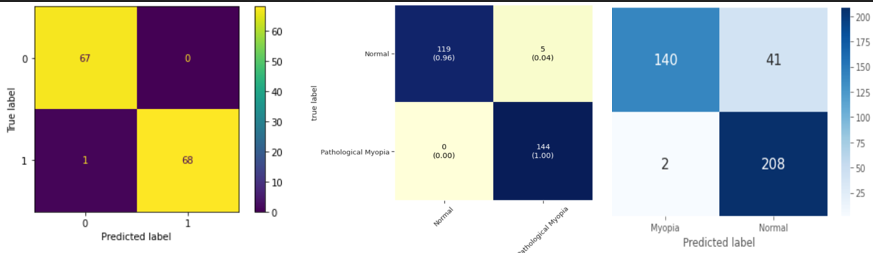
\includegraphics[scale=0.7]{50_Chapter_5/MNC.png}
    \caption{Confusion Matrix for Myopia v Normal.(Left: Resnet50, Middle: VGG19, Right: Mobilenetv2 on Augmented data)}
    \label{MNC}
\end{figure}
\begin{figure}[H]
    \centering
    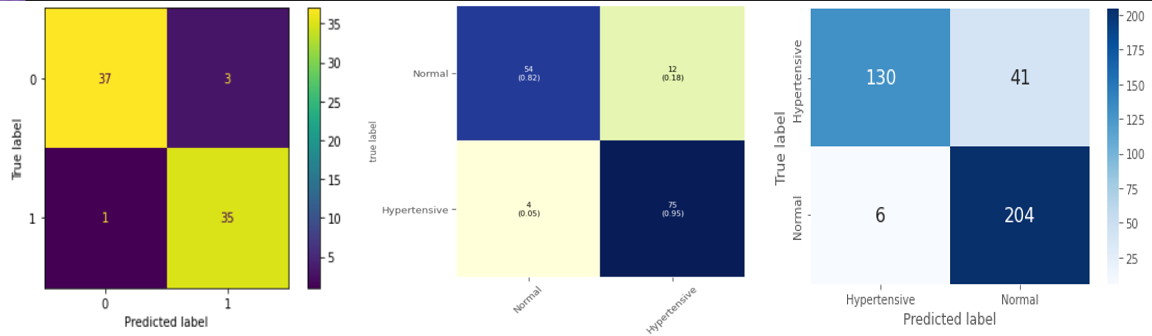
\includegraphics[scale=0.55]{50_Chapter_5/HNC.png}
    \caption{Confusion Matrix for Hypertensive v Normal.(Left: Resnet50, Middle: VGG19, Right: Mobilenetv2 on Augmented data)}
    \label{HNC}
\end{figure}
It is crucial to compare machine learning algorithms. Better performance of the machine learning software or solution is unquestionably the main goal of model comparison and selection. The goal is to select the fewest algorithms possible that meet the needs of the company and the data. If the chosen model fails to comprehend unknown input and is strongly associated with the training data, high performance may be short-lived. Finding a model that comprehends underlying data patterns is crucial in order to ensure that predictions are reliable and that little retraining is required. Minute details and information are captured when models are reviewed and prepared for comparisons, and they are useful during retraining.With the model information at hand, it is simple to focus on models that can provide fast processing and make efficient use of memory resources. Additionally, a number of parameters must be configured for the machine learning solutions throughout production.\\
\begin{table}[H]
\caption{MobileNetV2's Results Report without Augmented Data}
    \centering
    \begin{tabular}{|l|l|l|}
    \hline
        Model &  Accuracy \\ \hline
        Normal VS Cataract &  77\% \\ \hline
        Normal VS Glaucoma &  59\% \\ \hline
        Normal VS Myopia & 77\% \\ \hline
        Normal VS Hypertensive &  52\% \\ \hline
    \end{tabular}
\end{table}
\begin{table}[H]
\caption{Resnet50's Classification Report}
\centering
\begin{tabular}{|l|l|l|l|l|l|} 
\hline
Model                               & Accuracy                 & Disease              & Precision            & F1-score             & Recall                \\ 
\hline
\multirow{2}{*}{Normal VS Cataract} & \multirow{2}{*}{99.45\%} & Normal               & 0.98                 & 0.98                 & 0.98                  \\ 
\cline{3-6}
                                    &                          & Cataract             & 0.97                 & 0.97                 & 0.97                  \\ 
\hline
\multirow{2}{*}{Normal VS Glaucoma} & \multirow{2}{*}{90.98\%} & Normal               & 0.92                 & 0.91                 & 0.91                  \\ 
\cline{3-6}
                                    &                          & Glaucoma             & 0.9                  & 0.9                  & 0.91                  \\ 
\hline
Normal VS                           & \multirow{2}{*}{99.26\%} & Normal               & 0.99                 & 0.99                 & 1                     \\ 
\cline{3-6}
Myopia                              &                          & Myopia               & 1                    & 0.99                 & 0.99                  \\ 
\hline
Normal VS                           & \multirow{2}{*}{94.73\%} & Normal               & 0.97                 & 0.95                 & 0.93                  \\ 
\cline{3-6}
Hypertensive                        &                          & Hypertensive         & 0.92                 & 0.95                 & 0.97                  \\ 
\hline
\multicolumn{1}{l}{}                & \multicolumn{1}{l}{}     & \multicolumn{1}{l}{} & \multicolumn{1}{l}{} & \multicolumn{1}{l}{} & \multicolumn{1}{l}{} 
\end{tabular}
\end{table}
\begin{table} [H]
\caption{VGG19's Classification Report}
\centering
\begin{tabular}{|l|l|l|l|l|l|} 
\hline
Model                               & Accuracy                 & Disease              & Precision            & F1-score             & Recall                \\ 
\hline
\multirow{2}{*}{Normal VS Cataract} & \multirow{2}{*}{97.24\%} & Normal               & 0.94                 & 0.97                 & 1                     \\ 
\cline{3-6}
                                    &                          & Cataract             & 1                    & 0.97                 & 0.95                  \\ 
\hline
\multirow{2}{*}{Normal VS Glaucoma} & \multirow{2}{*}{90.94\%} & Normal               & 0.96                 & 0.89                 & 0.84                  \\ 
\cline{3-6}
                                    &                          & Glaucoma             & 0.88                 & 0.92                 & 0.997                 \\ 
\hline
Normal VS                           & \multirow{2}{*}{98.13\%} & Normal               & 1                    & 0.98                 & 0.96                  \\ 
\cline{3-6}
Myopia                              &                          & Myopia               & 0.97                 & 0.98                 & 1                     \\ 
\hline
Normal VS                           & \multirow{2}{*}{88.96\%} & Normal               & 0.97                 & 0.95                 & 0.93                  \\ 
\cline{3-6}
Hypertensive                        &                          & Hypertensive         & 0.92                 & 0.95                 & 0.97                  \\ 
\hline
\multicolumn{1}{l}{}                & \multicolumn{1}{l}{}     & \multicolumn{1}{l}{} & \multicolumn{1}{l}{} & \multicolumn{1}{l}{} & \multicolumn{1}{l}{} 
\end{tabular}
\end{table}
\begin{table}[H]
\caption{MobileNetV2's Classification Report with Augmented Data}
\centering
\begin{tabular}{|l|l|l|l|l|l|} 
\hline
Model                               & Accuracy                 & Disease              & Precision            & F1-score             & Recall                \\ 
\hline
\multirow{2}{*}{Normal VS Cataract} & \multirow{2}{*}{89.53\%} & Normal               & 0.85                 & 0.91                 & 0.98                  \\ 
\cline{3-6}
                                    &                          & Cataract             & 0.97                 & 0.88                 & 0.81                  \\ 
\hline
\multirow{2}{*}{Normal VS Glaucoma} & \multirow{2}{*}{84.00\%} & Normal               & 0.81                 & 0.86                 & 0.9                   \\ 
\cline{3-6}
                                    &                          & Glaucoma             & 0.88                 & 0.82                 & 0.77                  \\ 
\hline
Normal VS                           & \multirow{2}{*}{89.00\%} & Normal               & 0.84                 & 0.91                 & 0.99                  \\ 
\cline{3-6}
Myopia                              &                          & Myopia               & 0.99                 & 0.87                 & 0.77                  \\ 
\hline
Normal VS                           & \multirow{2}{*}{87.66\%} & Normal               & 0.83                 & 0.9                  & 0.97                  \\ 
\cline{3-6}
Hypertensive                        &                          & Hypertensive         & 0.96                 & 0.85                 & 0.76                  \\ 
\hline
\multicolumn{1}{l}{}                & \multicolumn{1}{l}{}     & \multicolumn{1}{l}{} & \multicolumn{1}{l}{} & \multicolumn{1}{l}{} & \multicolumn{1}{l}{} 
\end{tabular}
\end{table}
